%%%%%%%%%%%%%%%%%%%%%%%%%%%%%%%%%%%%%%%%%%%%%%%%%%%%%%%%%%%%%%%%%%%%%%%%%%%%%%%%%%%%%%%%%%%%%%%%%%%%%
% DOCUMENT CLASS
%%%%%%%%%%%%%%%%%%%%%%%%%%%%%%%%%%%%%%%%%%%%%%%%%%%%%%%%%%%%%%%%%%%%%%%%%%%%%%%%%%%%%%%%%%%%%%%%%%%%%%

\documentclass[journal=jacsat,manuscript=article]{achemso}

% Single-spaced, two-column with PRL look and style (easy on the eyes)
%\documentclass[aps,pre,twocolumn,superscriptaddress]{revtex4-1}
%\documentclass[aps,pre,twocolumn,superscriptaddress]{revtex4}

% Double-spaced, one-column style (for submission/review/editing)
%\documentclass[aps,preprint,prl,superscriptaddress,showpacs]{revtex4}

%%%%%%%%%%%%%%%%%%%%%%%%%%%%%%%%%%%%%%%%%%%%%%%%%%%%%%%%%%%%%%%%%%%%%%%%%%%%%%%%%%%%%%%%%%%%%%%%%%%%%%
% PREAMBLE
%%%%%%%%%%%%%%%%%%%%%%%%%%%%%%%%%%%%%%%%%%%%%%%%%%%%%%%%%%%%%%%%%%%%%%%%%%%%%%%%%%%%%%%%%%%%%%%%%%%%%%

\usepackage{palatino}
\usepackage{amsmath}
\usepackage{amssymb}
\usepackage{graphicx}
\usepackage{dcolumn}
\usepackage{boxedminipage}
\usepackage{verbatim}
\usepackage{booktabs}

\usepackage[colorlinks=true,citecolor=blue,linkcolor=blue]{hyperref}

% The figures are in a figures/ subdirectory.
\graphicspath{{../figures/}}

%\bibliographystyle{apsrevlong}
\bibliographystyle{apsrev}

% italicized boldface for math (e.g. vectors)
\newcommand{\bfv}[1]{{\mbox{\boldmath{$#1$}}}}
% non-italicized boldface for math (e.g. matrices)
\newcommand{\bfm}[1]{{\bf #1}}          

%\newcommand{\bfm}[1]{{\mbox{\boldmath{$#1$}}}}
%\newcommand{\bfm}[1]{{\bf #1}}
\newcommand{\expect}[1]{\left \langle #1 \right \rangle}                % <.> for denoting expectations over realizations of an experiment or thermal averages
\newcommand{\dhdl}{\frac{dH}{d\lambda}}
% vectors
\newcommand{\var}[1]{{\mathrm var}{(#1)}}
\newcommand{\x}{\bfv{x}}
\newcommand{\y}{\bfv{y}}
\newcommand{\f}{\bfv{f}}

\newcommand{\bfc}{\bfm{c}}
\newcommand{\hatf}{\hat{f}}

\newcommand{\bTheta}{\bfm{\Theta}}
\newcommand{\btheta}{\bfm{\theta}}
\newcommand{\bhatf}{\bfm{\hat{f}}}
\newcommand{\Cov}[1] {\mathrm{cov}\left( #1 \right)}
\newcommand{\Ept}[1] {{\mathrm E}\left[ #1 \right]}
\newcommand{\Eptk}[2] {{\mathrm E}_{#1}\left[ #2\right]}
\newcommand{\T}{\mathrm{T}}                                % T used in matrix transpose


\title{Benchmarking Simulations against the ThermoML Database: Neat Liquid Densities and Static Dielectrics}

 \author{Kyle A. Beauchamp$^*$}
 \affiliation{Memorial Sloan-Kettering Cancer Center, New York, NY}

 \author{Julie M. Behr$^*$}
 \affiliation{Memorial Sloan-Kettering Cancer Center, New York, NY}

\author{Patrick B. Grinaway }
 \affiliation{Memorial Sloan-Kettering Cancer Center, New York, NY}

\author{Bas}
 \affiliation{Memorial Sloan-Kettering Cancer Center, New York, NY}
 
 \author{Michael R. Shirts}
 \affiliation{Department of Chemical Engineering, University of Virginia, Charlottesville, VA}

 \author{Kenneth Kroenlein}
 \affiliation{NIST Thermodynamics Research Center, Boulder, CO}
 
 \author{John D. Chodera}
 \email{john.chodera@choderalab.org}
 \affiliation{Memorial Sloan-Kettering Cancer Center, New York, NY}



\begin{document}


\maketitle


\section{Abstract}

Useful atomistic simulations require accurate depictions of solvent.  Simple experimental observables, such as density and static dielectric constants, offer straightforward targets for evaluating forcefield quality.  Here we examine the possibility of benchmarking atomistic models against the NIST ThermoML database of physicochemical measurements, which curates thousands of density, dielectric, and other measurements.  We present a detailed benchmark of the GAFF forcefield against measurements extracted from ThermoML and discuss the extent of available data for neat liquids.  We show that empirical polarizability models correct systematic biases inherent in predicting dielectric constants with fixed-charged forcefields.  Combining our dataset with the Virtual Chemistry benchmark set provides an extensive benchmark suite for liquid properties.  

\section{Introduction}

Intro

\section{Results}

\subsection{Neat Liquid Measurements in ThermoML}

We performed a number of queries to summarize the ThermoML content relevant for benchmarking organic molecule forcefields.  Our aim is to explore neat liquid data with functional groups relevant to drug-like molecules.  We therefore applied the following sequence of filters: has either density or static dielectric measurements, contains a single component, contains only druglike elements (H, N, C, O, S, P, F, Cl, Br), has low heavy atom count $(\le 10)$, has ambient temperature [K] $(270 \le T \le 330)$, and has ambient pressure [kPA] $(100 \le P \le 102)$.  After applying these filters, we also assume that all pressures within this range are one atmosphere.  We also assume that temperatures can be rounded to one decimal place.  These approximations are motived by common data entry errors; for example, an experiment performed at water's freezing point at ambient pressure might be entered as either 101.325 kPA or 100 kPA, with a temperature of either 273 K or 273.15 K.  After the application of these filters (Table \ref{table:ThermoMLSummary}), we are left with 3591 densities and 432 static dielectrics--or 245 measurements for which both density and dielectric data are available.  

\begin{table}
\begin{tabular}{lrr}
\toprule
Filter &  Mass Density &  Static Dielectric \\
\midrule
0.  Single Component   &               130074 &                                     1649 \\
1.  Druglike Elements  &               120410 &                                     1649 \\
2.  Heavy Atoms        &                67897 &                                     1567 \\
3.  Temperature        &                36827 &                                      962 \\
4.  Pressure           &                13598 &                                      461 \\
5.  Aggregate T, P     &            \bf{3591} &                                 \bf{432} \\
6.  Density+Dielectric &             \bf{245} &                                 \bf{245} \\
\bottomrule
\end{tabular}
\caption{ThermoML Statistics}
\label{table:ThermoMLSummary}
\end{table}

%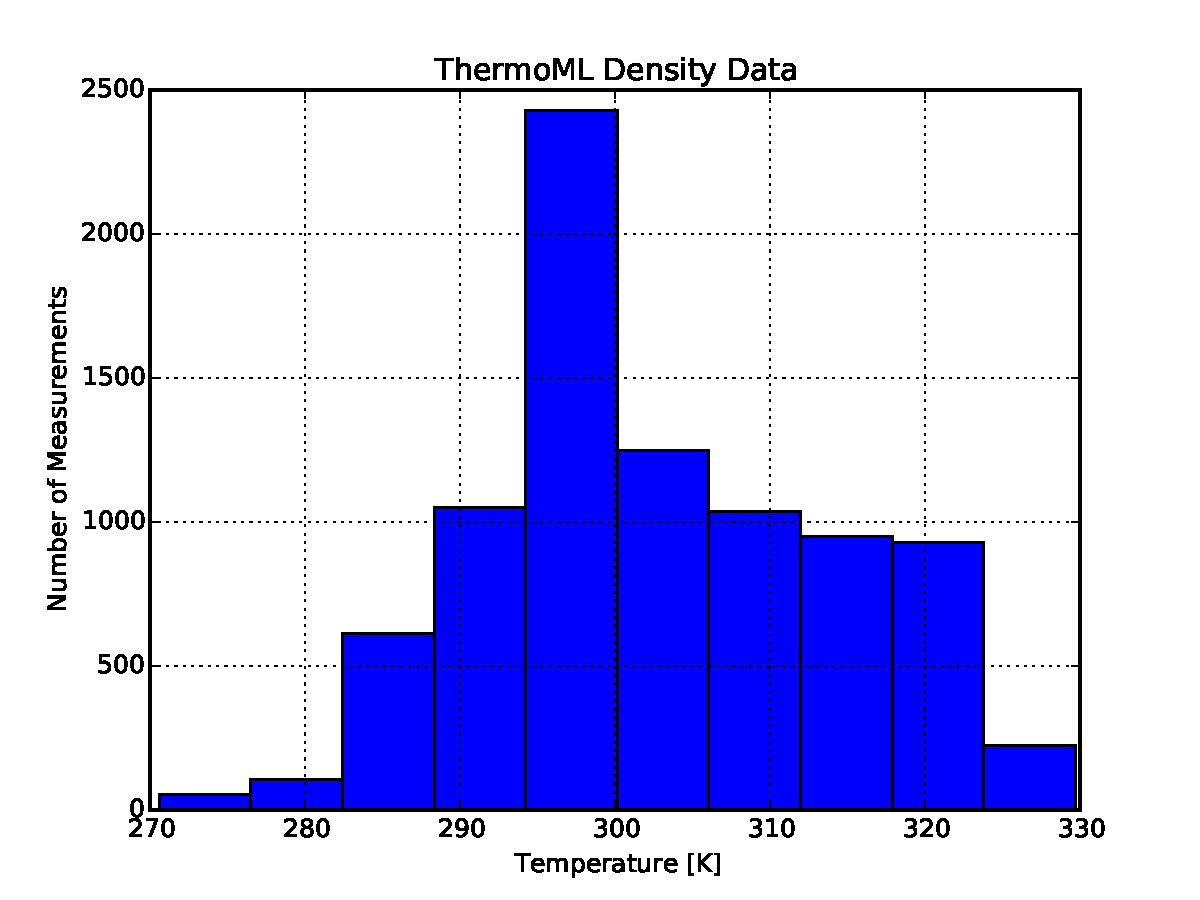
\includegraphics[width=\columnwidth]{./figures/thermoml_density_histogram.pdf}

\subsection{Benchmarking GAFF against ThermoML: Mass Density}

Mass density has been widely used as a critical ingredient for parameterizing and testing forcefields, particularly the Lennard Jones parameters.  We therefore used the present ThermoML compilation as a benchmark of the Generalized Amber Force Field.  

\begin{figure}
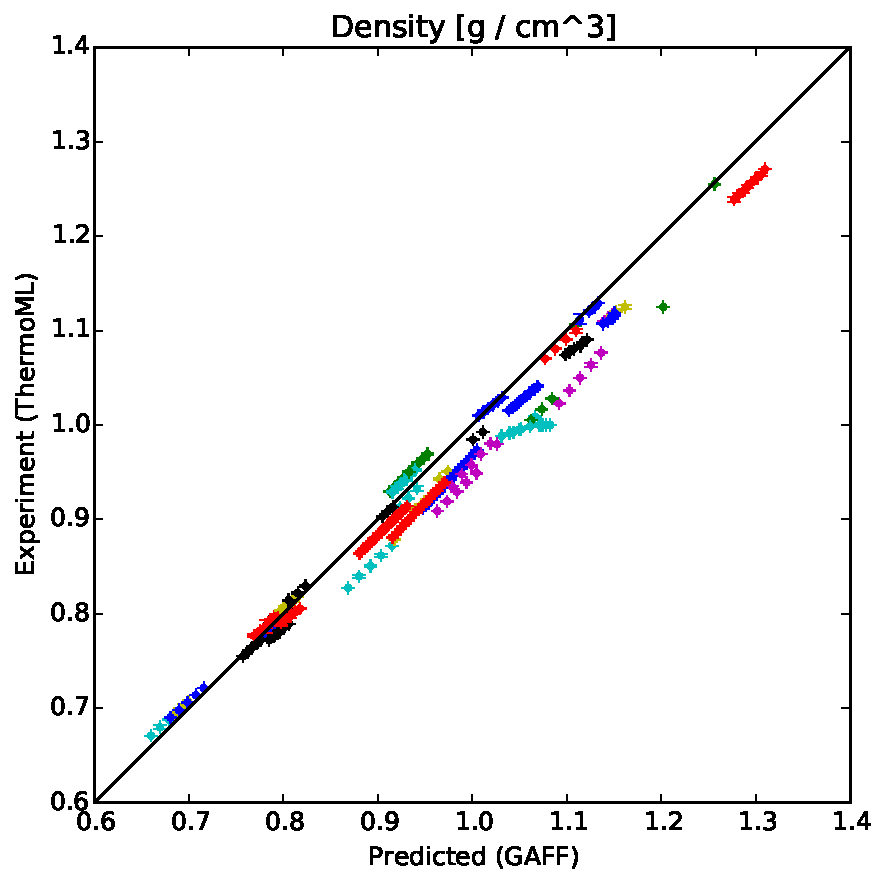
\includegraphics[width=\columnwidth]{./figures/densities_thermoml.pdf}
\caption{Measured (ThermoML) versus predicted (GAFF) densities.  Color groupings represent identical chemical formulas.  Simulation error bars represent one standard error of the mean, with the number of effective (uncorrelated) samples estimated using pymbar.  Experimental error bars indicate the standard deviation between independently reported measurements, when available, or the authors reported standard deviations; for some measurements, neither uncertainty estimate is available.  
}
\end{figure}


\subsection{Benchmarking GAFF against ThermoML: Static Dielectric}

As a measure of the electronic medium, the static dielectric constant of neat liquids provides a critical benchmark that is orthogonal to density and thermodynamic quantities.  We therefore compare our GAFF simulations against the measurements in our ThermoML compilation.  Overall, we find the dielectric constants to be qualitatively reasonable, but with clear deviations from experiment.  In particular, the nonpolar organics show a clear discrepancy, with the GAFF predictions of 1.0 being substantially less polar than the measurements near 2.0.  Because this deviation likely stems from the lack of electronic polarization, we added a simple empirical correction for polarization \cite{bosque2002polarizabilities}, which leads to better agreement with experiment.  A similar polarization correction was used in the development of the TIP4P-EW water model \cite{horn2004}; however, the need is much greater for the nonpolar organics, as the missing polarizability is the dominant contribution to the static dielectric constant.  For comparison, we also applied the same empirical correction to the VirtualChemistry dataset \cite{caleman2011force, van2012gromacs} and saw similarly improved agreement with experiment for both the GAFF and OPLS forcefields.


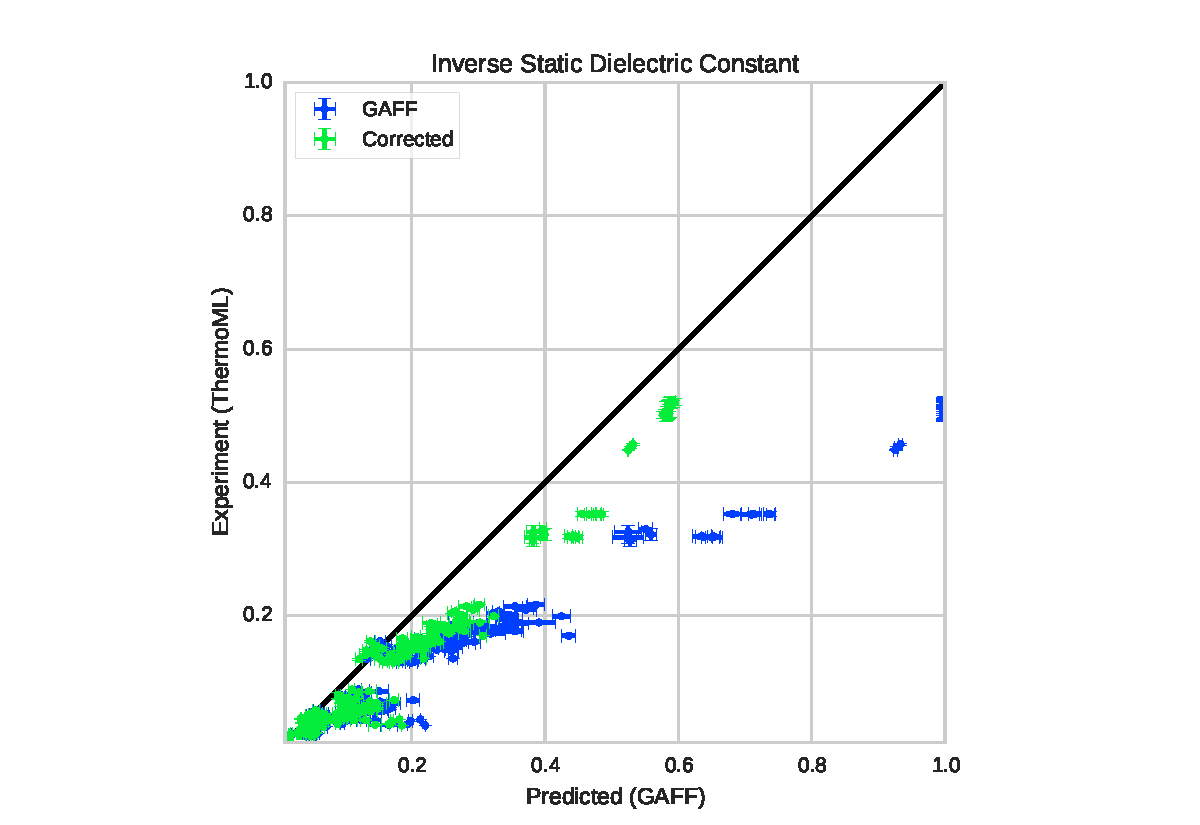
\includegraphics[width=\columnwidth]{./figures/dielectrics_thermoml.pdf}

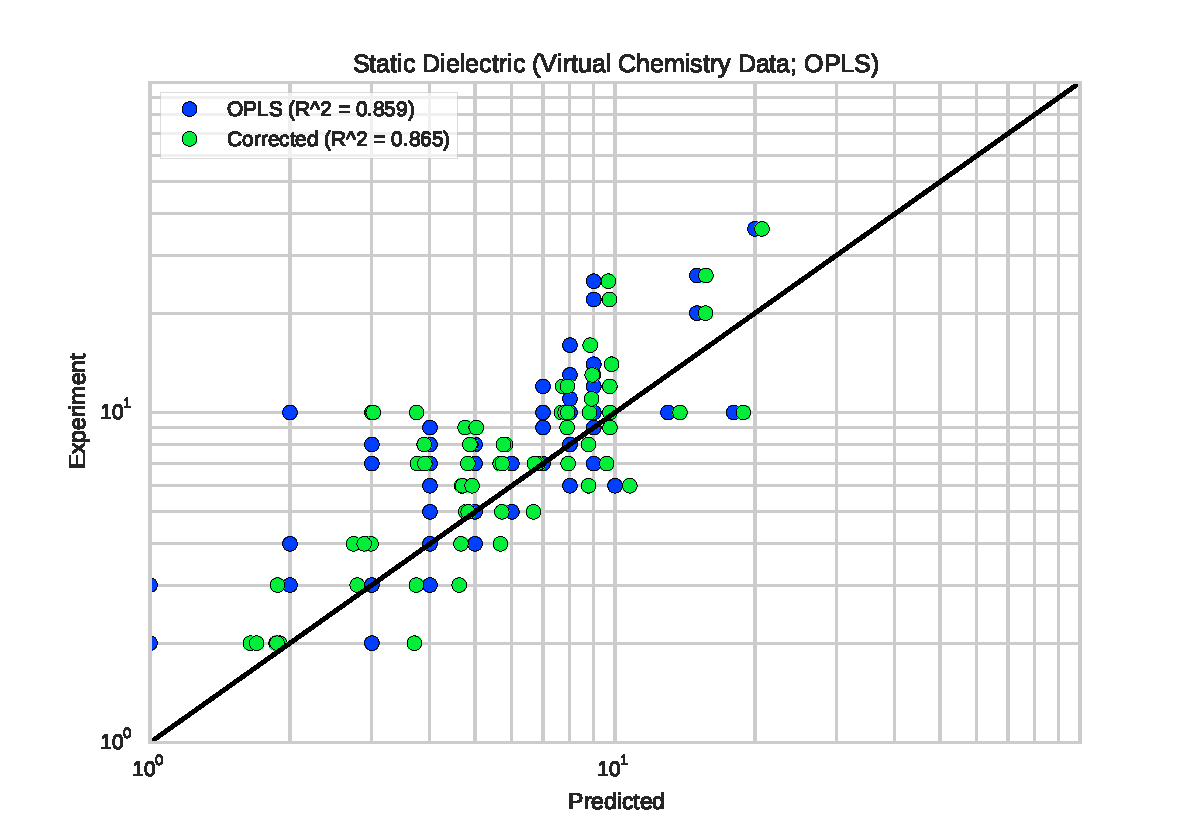
\includegraphics[width=\columnwidth]{./figures/dielectric_virtual_chemistry_opls.pdf}

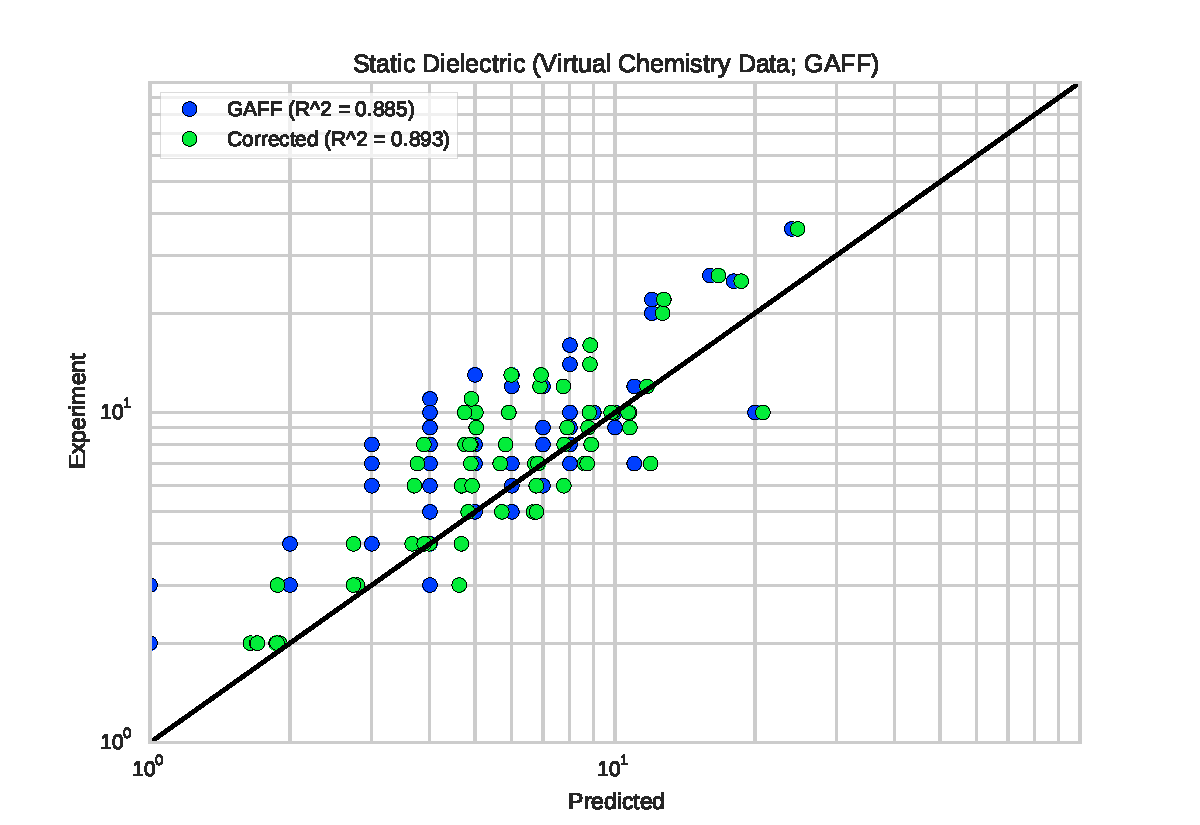
\includegraphics[width=\columnwidth]{./figures/dielectric_virtual_chemistry_gaff.pdf}

\section{Discussion}

\subsection{Forcefield Accuracy Depends on Functional Group}

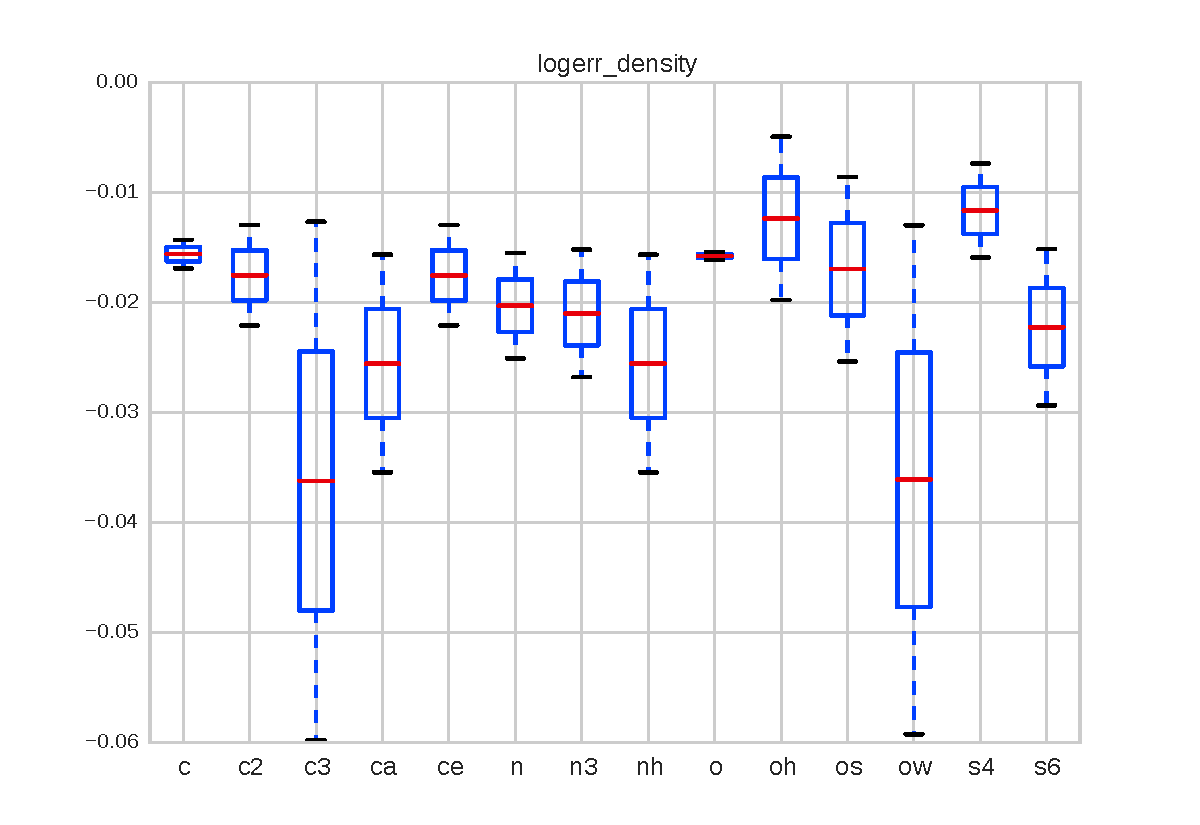
\includegraphics[width=\columnwidth]{./figures/functional_group_logerr_density.pdf}

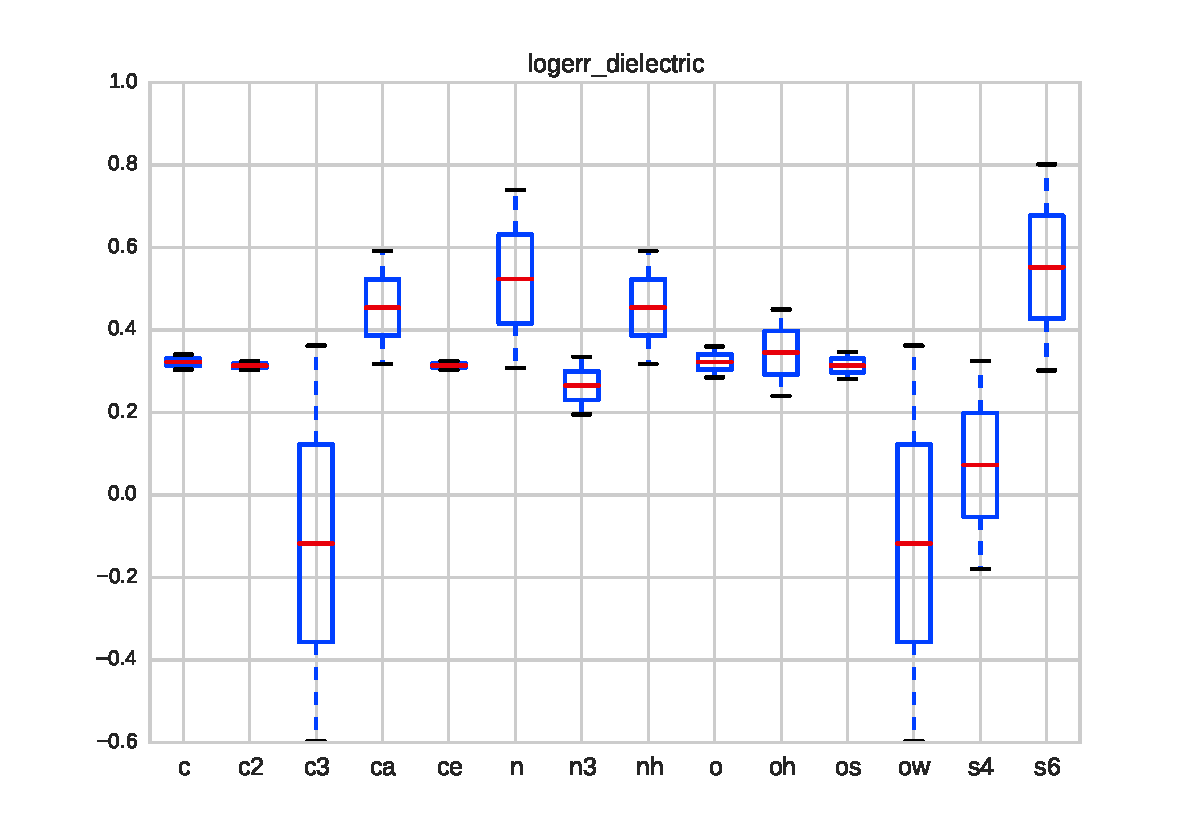
\includegraphics[width=\columnwidth]{./figures/functional_group_logerr_dielectric.pdf}

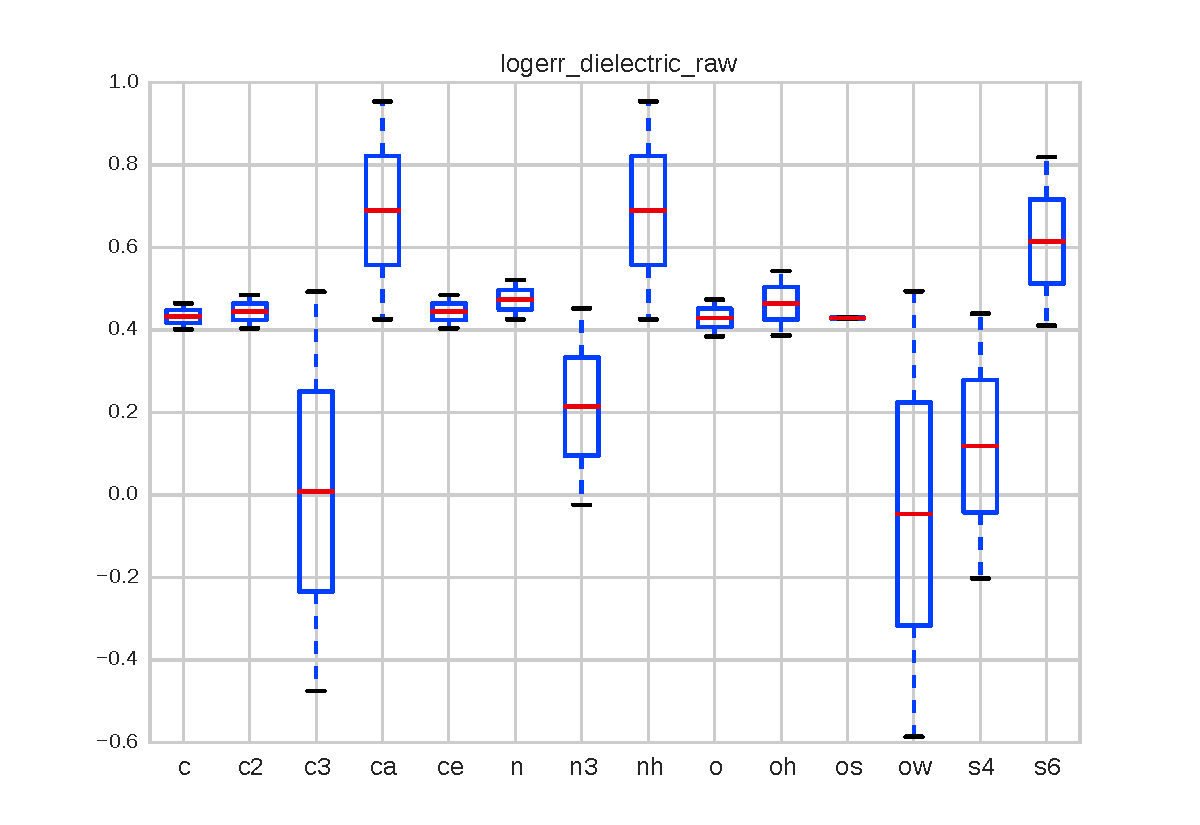
\includegraphics[width=\columnwidth]{./figures/functional_group_logerr_dielectric_raw.pdf}

\subsection{Fitting Forcefields to Dielectric Constants}

Recent forcefield development has seen a resurgence of papers fitting dielectric constants as primary data \cite{wang2014building, fennell2014fixed}.  However, a number of authors have pointed out potential challenges in constructing self-consistent fixed-charge force fields \cite{fennell2012simple, leontyev2014polarizable}.  Interestingly, a recent work by Dill \cite{fennell2012simple} pointed out that, for $\mathrm{CCl_4}$, reasonable choices of point charges are incapable of recapitulating the observed dielectric of 2.2, instead producing dielectric constants in the range of $1.0 \le \epsilon \le 1.05$.  Suppose, for example, that one attempts to directly fit the static dielectric constants of $\mathrm{CCl_4}$, $\mathrm{CHCl_3}$, $\mathrm{CH_2Cl_2}$, $\mathrm{CH_3Cl_1}$, $\mathrm{CH_4}$.  In moving from the tetrahedrally-symmetric $\mathrm{CCl_4}$ to $\mathrm{CHCl_3}$, it suddenly becomes possible to achieve the observed dielectric constant of 4.8.  However, the model for $\mathrm{CHCl_3}$ uses fixed point charges to account for \emph{both} the net dipole moment and the (electronic) polarizability, whereas the $\mathrm{CCl_4}$ model contains no treatment of polarizability.  We hypothesize that this inconsistency in parameterization may lead to strange mismatches, where symmetric molecules (e.g. benzene, $\mathrm{CCl_4}$) have qualitatively different properties than closely related asymmetric molecules (e.g. toluene, $\mathrm{CHCl_3}$).  As a first-order fix, we suggest using empirical polarization corrections before directly comparing measured static dielectric constants to fixed-charge models---particularly when examining low-dielectric solvents.  Separating the contributions of fixed charges and polarization may also lead to the development of improved models of electrostatics that account for the missing polarization physics.


\subsection{ThermoML as a Data Source}

The present work has focused on the neat liquid density and dielectric measurements present in ThermoML \cite{frenkel2006xml, frenkel2003thermoml, chirico2003thermoml} as a target for molecular dynamics forcefield validation.  While densities and dielectric constants have been widely used in forcefield work, several aspects of ThermoML make it a unique resource for the forcefield community.  First, the curation, support, and dissemination of ThermoML is supported by NIST, whose mission makes these tasks a long-term priority.  Second, ThermoML is actively growing, through partnerships with journals such as J. Chem. Thermo--new experimental measurements published in these journals are critically examined by the TRC and included in the archive.  Finally, the files in ThermoML are machine readable via a formal XML schema, allowing facile access to thousands of measurements.  In the future, we hope to examine additional measurement classes, including both mixture and two-phase data.


\section{Methods}

\subsection{ThermoML Processing}

ThermoML XML files were obtained from the the NIST TRC.  To explore their content, we created a python (version 2.7.9) tool (ThermoPyl: \url{https://github.com/choderalab/ThermoPyL}) that munges the XML content into spreadsheet-like format accessible via the  Pandas (version 0.15.2) library.  First, we obtained the XML schema (\url{http://media.iupac.org/namespaces/ThermoML/ThermoML.xsd}) defining the layout of the data.  This scheme was converted into a Python object via PyXB 1.2.4 (\url{http://pyxb.sourceforge.net/}).  Finally, the scheme was used to extract the data.  

\subsection{Simulation}
Boxes of 1000 molecules were constructed using PackMol \cite{martinez2009packmol}.  AM1-BCC charges were generated using OpenEye toolkit 2014-6-6 \cite{openeye}, using the XYZ module with parameter ZYX.  The selected conformer was then processed using antechamber in AmberTools 14.  The resulting AMBER files were converted to OpenMM \cite{eastman2012openmm} XML files.  Simulation code used libraries gaff2xml 0.1, TrustButVerify 0.1, openmm 6.2, and MDTraj \cite{mcgibbon2014mdtraj} 1.2.  

Molecular dynamics simulations were performed using OpenMM 6.2 using a Langevin integrator (friction $1 ps^{-1}$) and a 1 fs timestep; interestingly, we found that a 2 fs timestep led to insufficient accuracy in equilibrium densities (Fig. S1).  Pressure coupling was achieved with a Monte Carlo barostat applied every 25 steps.  Particle mesh Ewald \cite{Darden1993} was used with a long-range cutoff of 0.95 nm and an isotropic dispersion correction.  Simulations were continued until density standard errors were less than $2 \times 10^{-4}$ g / mL, as estimated using the equilibration detection module in pymbar 2.1 \cite{shirts2008statistically}.  Trajectory analysis was performed using OpenMM \cite{eastman2012openmm} and MDTraj \cite{mcgibbon2014mdtraj}.  

\section{Conclusions}

1.  ThermoML is a potentially useful resource for the forcefield community
2.  We have curated a subset of ThermoML for neat liquids with druglike atoms, with thousands of densities and hundreds of dielectrics
3.  Empirical polarization models correct a systematic bias in comparing fixed-charge forcefields to static dielectric constants


\section{Acknowledgements}

We thank Vijay Pande, Lee-Ping Wang, Peter Eastman, Robert McGibbon, Jason Swails, David Mobley, Christopher Bayly, and members of Chodera lab for helpful discussions.  

\section{Supplementary Information}

\begin{table}
\begin{tabular}{lrrrrrrr}
\toprule
{} &        mu &       n &          neff &     sigma &    stderr &     error &    relerr \\
\midrule
0.5 &  0.903701 &  145510 &  20357.973571 &  0.007362 &  0.000052 &  0.000000 &  0.000000 \\
1.0 &  0.903114 &  159515 &  21988.457281 &  0.007415 &  0.000050 & -0.000588 & -0.000650 \\
2.0 &  0.901811 &  108346 &  15964.072327 &  0.007494 &  0.000059 & -0.001891 & -0.002092 \\
\bottomrule
\end{tabular}
\caption{To probe the systematic error from finite time-step integration, we examined the timestep dependence of butyl acrylate density.  The number of effective samples was estimated using pymbar's statistical inefficiency routine \cite{shirts2008statistically}.  To approximate the timestep bias, we compare the density expectation ($\langle \rho \rangle$) to values calculated with a 0.5fs timestep.  We find a 2fs timestep leads to systematic biases in the density on the order of 0.2\%, while 1fs reduces the systematic bias to less than 0.1\%---we therefore selected a 1fs timestep for the present work, where we aimed to achieve three digits of accuracy in density predictions.
}
\label{table:TimestepDependence}
\end{table}


\bibliography{benchmark}

\end{document}